\documentclass[11pt]{beamer}

\usepackage[utf8]{inputenc}  
\usepackage{polski}
\usepackage{animate}
\usepackage{amsmath}
\usepackage{algorithmic}
\usepackage{float}
\usepackage{array}
\usepackage{algorithm}
\usepackage{textpos}
\usepackage{caption}
\usepackage{multicol}
\usepackage{beamerthemesplit}
\usepackage{braket, booktabs}
\usepackage{xcolor}

\usetheme{Warsaw}

\newcommand{\backupbegin}{
   \newcounter{finalframe}
   \setcounter{finalframe}{\value{framenumber}}
}
\newcommand{\backupend}{
   \setcounter{framenumber}{\value{finalframe}}
}

\newcommand{\zerodisplayskips}{%
  \setlength{\abovedisplayskip}{0pt}%
  \setlength{\belowdisplayskip}{0pt}%
  \setlength{\abovedisplayshortskip}{0pt}%
  \setlength{\belowdisplayshortskip}{0pt}}
\appto{\normalsize}{\zerodisplayskips}
\appto{\small}{\zerodisplayskips}
\appto{\footnotesize}{\zerodisplayskips}

\definecolor{darkpowderblue}{rgb}{0.0, 0.2, 0.6}
\definecolor{lasallegreen}{rgb}{0.03, 0.47, 0.19}

\DeclareMathOperator*{\argmax}{arg\,max}
\newtheorem{lem}{Lemma}
\author{Stanisław Wilczyński}
\title[Analiza mikromacierzy DNA - egzamin magisterski]{Analiza mikromacierzy DNA w predykcji występowania przerzutów raka piersi}
%\setbeamercovered{transparent} 
\addtobeamertemplate{navigation symbols}{}{%
    \usebeamerfont{footline}%
    \usebeamercolor[fg]{footline}%
    \hspace{1em}%
    \insertframenumber/\inserttotalframenumber
}
\def\bz{{\bf Z}}
\def\Errhat{\widehat{\rm Err}}
\institute{\textbf{Promotor:} dr. Jan Chorowski\\ \ \\Uniwersytet Wrocławski\\Wydział Matematyki i Informatyki\\Instytut Informatyki} 
\date{20.09.2019} 
%\subject{} 

\begin{document}


\begin{frame}
\titlepage
\end{frame}

\begin{frame}{Wstęp}
\begin{itemize}
    \item Mnóstwo prac poświęconych klasyfikacji guzów i predykcji rozwoju choroby
    \item \textbf{Cel:} redukcja liczby pacjentów wysłanych niepotrzebnie na chemioterapię
    \item Mikromacierze jako innowacyjna metoda badań medycznych dostarczająca ogromne ilości danych
    \item Interesujący, mniej popularny obszar klasyfikacji ($n \ll p$)
    \item Analiza i porównanie nowatorskich oraz standardowych metod używanych w literaturze
    \item Kontynuacja badań z pracy licencjackiej
\end{itemize}
\end{frame}

\begin{frame}{Biologiczny kontekst}
\begin{columns}[t]
\begin{column}{0.49\linewidth}
\begin{itemize}
    \item DNA złożone z genów ulega ekspresji tworząc białka
    \item Poziom ekspresji - ilość produktu
    \item Mikromacierze DNA - zróżnicowane technologie mierzenia poziomu ekspresji
    \item Guzy i przerzuty
    \item Użyte dane - połączone 10 zbiorów z Gene Expression Omnibus ($969 \times 12179$)
\end{itemize} 
\end{column}
\begin{column}{0.49\linewidth}
\begin{figure}
\centering
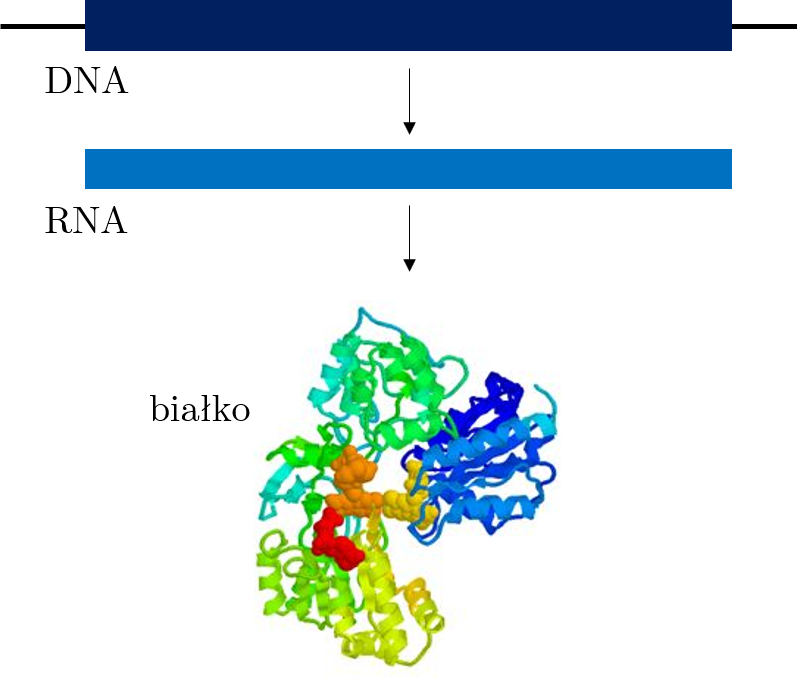
\includegraphics[width=0.9\textwidth]{images/ekspresja.png}
\caption{Schemat ekspresji genów}
\end{figure}
\end{column}
\end{columns}
\end{frame}

\begin{frame}{Wstępna analiza danych (EDA)}

\begin{itemize}
    \item Badanie podstawowych statystyk (skośność + kurtoza)
    \item Analiza rozkładów poszczególnych zmiennych
    \item Wpływ różnych rodzajów normalizacji
    \item Studium korelacji
\end{itemize}

\begin{block}<2->{Wniosek}
Wystarczająca zgodność z rozkładem normalnym, brak potrzeby dalszego preprocessingu
\end{block}
    
\end{frame}

\begin{frame}{Wykorzystane metody}

\begin{columns}[t]
\begin{column}{0.25\linewidth}
\textcolor{darkpowderblue}{\textbf{Regularyzowane klasyfikatory:}}
\begin{itemize}
    \item RF
    \item LR
    \item RDA
    \item NSC
    \item SVC
    \item \textbf{RLR}
\end{itemize}
\end{column}
\hfill

\begin{column}{0.35\linewidth}
\textcolor{lasallegreen}{\textbf{Ekstrakcja \\zmiennych:}}
\begin{itemize}
    \item Bez nadzoru
    \begin{itemize}
        \item PCA
        \item SPCA
        \item \textbf{MLCC}
    \end{itemize}
    \item Z nadzorem
    \begin{itemize}
    \item PLS
    \item FDNN
    \end{itemize}
    \end{itemize}
\end{column}
\hfill
    

\begin{column}{0.25\linewidth}
\textcolor{lasallegreen}{\textbf{Selekcja zmiennych:}}
\begin{itemize}
    \item SAM
    \item RFE
\end{itemize}
\end{column}
    
\end{columns}
\end{frame}


\begin{frame}{Modele wybrane za pomocą NCV}

\begin{figure}
\centering
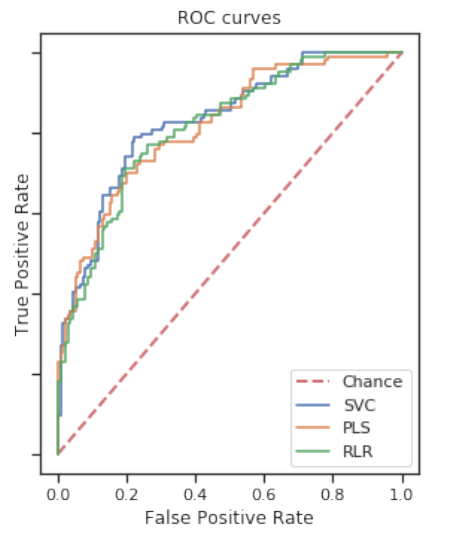
\includegraphics[width=0.53\textwidth]{images/rocTestCut.png}
\caption{Krzywe ROC dla PLS, SVC i RLR}
\end{figure}
\end{frame}

\begin{frame}{Analiza wyników}

\begin{itemize}
    \item Recall - $\frac{TP}{TP+FN}$
    \item Precision - $\frac{TP}{TP+FP}$
    \item ROC AUC - wartość recall uśredniona po progach FPR
\end{itemize}
\vspace{-4ex}

\begin{table}
\centering
    \begin{tabular}[t]{c c c c c}
    \toprule
    & ROC AUC & Prec (0.95) & Prec (0.8) & Acc (0.9)\\
    \midrule
    PLS & $0.818$ & $0.556$ & $0.596$ & $0.650$ \\
    SVC & $0.831$ & $0.515$ & $0.689$ & \\
    RLR & $0.815$ & $0.527$ & $0.641$ & \\
    PCA-AE-Ada\footnotemark[1] & \only<2>{\color{red}}$0.714$ & & &  \\
    Protein Net\footnotemark[1] & & & & \only<2>{\color{red}}$0.558$ \\
    \bottomrule
\end{tabular}
    \caption{Metryki dla wybranych metod, (wartość recall)}
\end{table}

% \begin{block}<2->{Wniosek}
%     Zaprezentowane metody działają skuteczniej od metod z literatury
% \end{block}
\footnotetext[1]{Dane literaturowe}
    
\end{frame}

\begin{frame}{Przewaga selekcji nad ekstrakcją}

\begin{itemize}
    \item Środowisko medyczne
    \begin{itemize}
        \item Brak akceptacji \textit{czarnych skrzynek}, jasne uzasadnienie diagnozy
    \end{itemize}
    \item Dodatkowe atuty
    \begin{itemize}
        \item Wskazanie konkretnych biomarkerów
        \item Odkrycie zależności pomiędzy genami, a nie binarna diagnoza
    \end{itemize}
\end{itemize}

\begin{block}<2->{Wniosek}
    Pomimo mniejszych wartości metryk klasyfikacji, selekcja może być bardziej odpowiednia dla zastosowań medycznych
\end{block}
    
\end{frame}

\begin{frame}{Selekcja zmiennych}
\begin{figure}
\centering
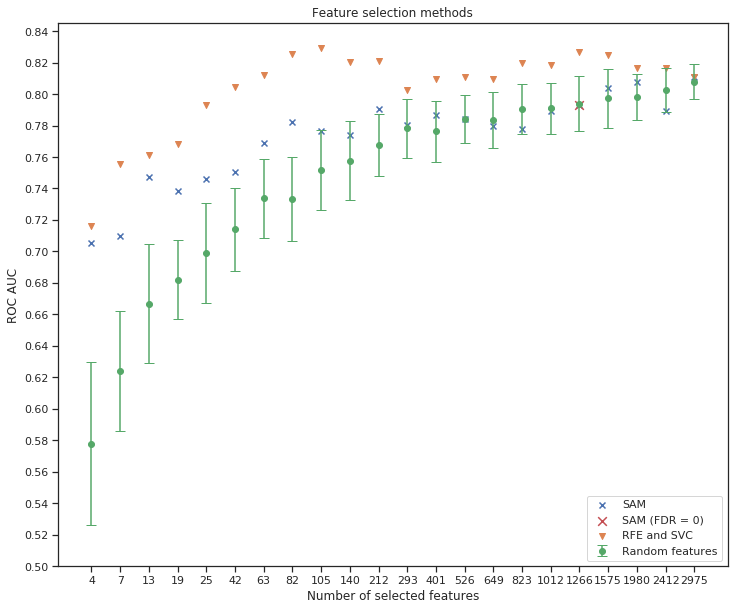
\includegraphics[width=0.77\textwidth]{images/selection-scores.png}
\caption{ROC AUC dla metod selekcji zmiennych}
\end{figure}
    
\end{frame}



\begin{frame}{Wnioski}
\begin{itemize}
\item Wybrana metoda - RFE z użyciem SVC (105 zmiennych)
    \begin{itemize}
        \item Wysokie ROC AUC
        \item Zalety selekcji przeważają
        \item \textbf{Wada:} brak zgodności w wybieranych zmiennych $\Rightarrow$ konieczność sprawdzenia przez specjalistę
    \end{itemize}
\item Konieczność współpracy statystyków i biologów:
\begin{itemize}
    \item Różnorodność (małych) zbiorów danych i wyników
    \item Brak dostępnego kodu źródłowego, wyniki niereprodukowalne
    \item Użycie tylko prostych modeli
    \item Brak wsparcia profesjonalnych statystyków
    \item Ewentualne uwzględnienie dodatkowych biomarkerów
    \item Weryfikacja wyników przez biologów
\end{itemize}
\item Narzędzie wspomagające diagnozę
\end{itemize}
\end{frame}


\appendix
\backupbegin
\begin{frame}[allowframebreaks]{Bibliografia}

{\tiny
\nocite{*}
\bibliography{biblio}
\bibliographystyle{plain}
}%
\end{frame}



\backupend
\end{document}